% begin module direction-fields-procedure
\begin{frame}
\frametitle{Direction Fields}
\begin{itemize}
\item  How do we sketch the graph of the solution to $y' = x + y$ that satisfies the initial condition $y(0) = 1$?
\item<2->  Make a table of values of $y'$.
\end{itemize}
\begin{columns}[c]

\column{.25\textwidth}
\uncover<2->{%
\[%
\begin{array}{|c|r|}
\hline
\textrm{Point} & y' \\
\hline
\alert<handout:0| 3-4>{(1,0)}&%
\alert<handout:0| 3-4>{\uncover<4->{1}}\\%
\alert<handout:0| 5-6>{(-1,0)}&%
\alert<handout:0| 5-6>{\uncover<6->{-1}}\\%
\alert<handout:0| 7-8>{(0,1)}&%
\alert<handout:0| 7-8>{\uncover<8->{1}}\\%
\alert<handout:0| 9-10>{(0,-1)}&%
\alert<handout:0| 9-10>{\uncover<10->{-1}}\\%
\alert<handout:0| 11-12>{(0,0)}&%
\alert<handout:0| 11-12>{\uncover<12->{0}}\\%
\alert<handout:0| 13-14>{(1,1)}&%
\alert<handout:0| 13-14>{\uncover<14->{2}}\\%
\alert<handout:0| 15-16>{(1,-1)}&%
\alert<handout:0| 15-16>{\uncover<16->{0}}\\%
\alert<handout:0| 17-18>{(-1,1)}&%
\alert<handout:0| 17-18>{\uncover<18->{0}}\\%
\alert<handout:0| 19-20>{(-1,-1)}&%
\alert<handout:0| 19-20>{\uncover<20->{-2}}\\%
\hline
\end{array}
\]%
}%


\column{.45\textwidth}
\psset{xunit=1cm, yunit=1cm}
\begin{pspicture}(-2.8,-2.8)(2.8,2.8)
\tiny
\fcAxesStandard{-2.7}{-2.7}{2.7}{2.7}%
%WARNING THE LATEX MESSES UP WHITE SPACE. DO NOT USE SPACES
\fcXTickWithLabel{1}{$1$}%
\fcXTickWithLabel{2}{$2$}%
\uncover<4-33>{%
\fcDirectionFieldOneTangent{x y add}{1}{0}{0.2}{0.02}{linecolor=blue}%
}%
\uncover<6-33>{%
\fcDirectionFieldOneTangent{x y add}{-1}{0}{0.2}{0.02}{linecolor=blue}%
}%
\uncover<8-33>{%
\fcDirectionFieldOneTangent{x y add}{0}{1}{0.2}{0.02}{linecolor=blue}%
}%
\uncover<10-33>{%
\fcDirectionFieldOneTangent{x y add}{0}{-1}{0.2}{0.02}{linecolor=blue}%
}%
\uncover<12-33>{%
\fcDirectionFieldOneTangent{x y add}{0}{0}{0.2}{0.02}{linecolor=blue}%
}%
\uncover<14-33>{%
\fcDirectionFieldOneTangent{x y add}{1}{1}{0.2}{0.02}{linecolor=blue}%
}%
\uncover<16-33>{%
\fcDirectionFieldOneTangent{x y add}{1}{-1}{0.2}{0.02}{linecolor=blue}%
}%
\uncover<18-33>{%
\fcDirectionFieldOneTangent{x y add}{-1}{1}{0.2}{0.02}{linecolor=blue}%
}%
\uncover<20-33>{%
\fcDirectionFieldOneTangent{x y add}{-1}{-1}{0.2}{0.02}{linecolor=blue}%
}%
\uncover<23>{%
\psline(-2.5,2.5)(2.5,-2.5)%
}%
\uncover<24>{%
\multido{\ra=-2.5+0.5}{11}{%
\fcDirectionFieldOneTangent{x y add}{\ra}{\ra\space -1 mul} {0.2}{0.02}{linecolor=red}%
}%
}%
\uncover<25-33>{%
\multido{\ra=-2.5+0.5}{11}{%
\fcDirectionFieldOneTangent{x y add}{\ra}{\ra\space -1 mul} {0.2}{0.02}{linecolor=blue}%
}%
}%
\uncover<25>{%
\psline(-2,2.5)(2.5,-2)%
}%
\uncover<26>{%
\multido{\ra=-2.5+0.5}{10}{%
\fcDirectionFieldOneTangent{x y add}{\ra\space 0.5 add}{\ra\space -1 mul} {0.2}{0.02}{linecolor=red}%
}%
}%
\uncover<27-33>{%
\multido{\ra=-2.5+0.5}{10}{%
\fcDirectionFieldOneTangent{x y add}{\ra\space 0.5 add}{\ra\space -1 mul} {0.2}{0.02}{linecolor=blue}%
}%
}%
\uncover<27>{%
\psline(-1.5,2.5)(2.5,-1.5)%
}%
\uncover<28>{%
\multido{\ra=-2.5+0.5}{9}{%
\fcDirectionFieldOneTangent{x y add}{\ra\space 1 add}{\ra\space -1 mul} {0.2}{0.02}{linecolor=red}%
}%
}%
\uncover<28-33>{%
\multido{\ra=-2.5+0.5}{9}{%
\fcDirectionFieldOneTangent{x y add}{\ra\space 1 add}{\ra\space -1 mul} {0.2}{0.02}{linecolor=blue}%
}%
}%
\uncover<29>{%
\psline(-2.5,2)(2,-2.5)%
}%
\uncover<30-33>{%
\multido{\ra=-2.5+0.5}{10}{%
\fcDirectionFieldOneTangent{x y add}{\ra}{\ra\space -1 mul 0.5 sub} {0.2}{0.02}{linecolor=red}%
}%
}%
\uncover<31-33>{%
\multido{\ra=-2.5+0.5}{10}{%
\fcDirectionFieldOneTangent{x y add}{\ra}{\ra\space -1 mul 0.5 sub} {0.2}{0.02}{linecolor=blue}%
}%
}%
\uncover<31>{%
\psline(-2.5,1.5)(1.5,-2.5)%
}%
\uncover<32>{%
\multido{\ra=-2.5+0.5}{9}{%
\fcDirectionFieldOneTangent{x y add}{\ra}{\ra\space -1 mul 1 sub} {0.2}{0.02}{linecolor=red}%
}%
}%
\uncover<33>{%
\multido{\ra=-2.5+0.5}{9}{%
\fcDirectionFieldOneTangent{x y add}{\ra}{\ra\space -1 mul 1 sub} {0.2}{0.02}{linecolor=blue}%
}%
}%
\uncover<34->{%
\fcDirectionFieldDefault{x y add}{-2.5}{-2.5}{0.5}{11}%
}%
\uncover<35->{%
%Function formula: 2 e^{x}- x-1
\psplot[linecolor=\fcColorGraph, plotpoints=1000]{-2.7}{0.814045}{-1 x -1 mul add 2.718281828 x exp 2 mul add }
}%
\end{pspicture}

%\ \only<handout:0| -3>{%
%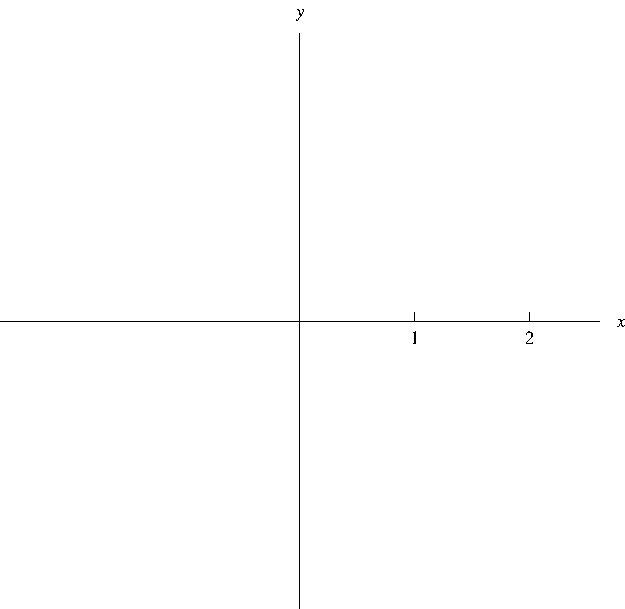
\includegraphics[height=5cm]{diff-eq-direction-fields/pictures/10-02-dirfielda.pdf}%
%}%
%\only<handout:0| 4>{%
%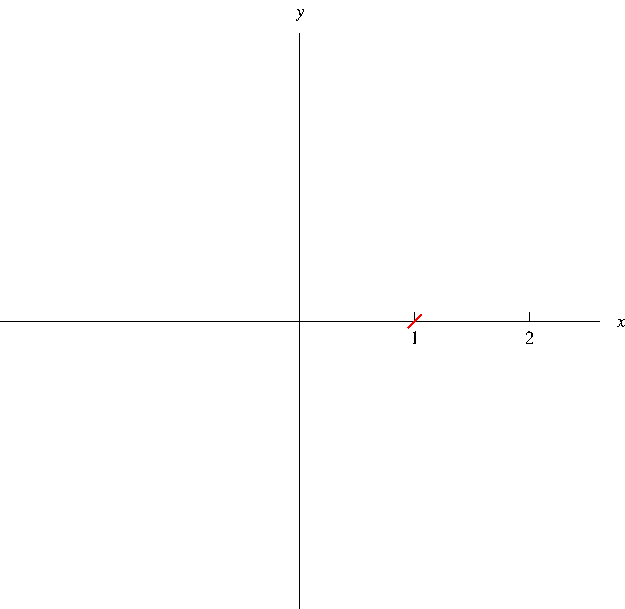
\includegraphics[height=5cm]{diff-eq-direction-fields/pictures/10-02-dirfieldb.pdf}%
%}%
%\only<handout:0| 5>{%
%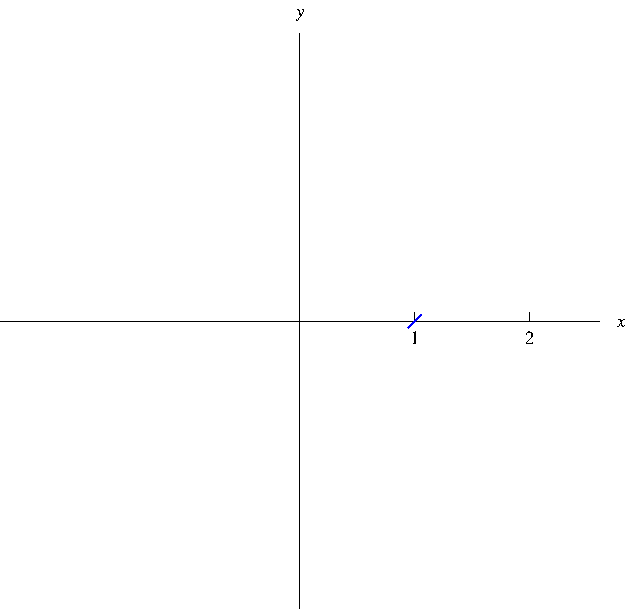
\includegraphics[height=5cm]{diff-eq-direction-fields/pictures/10-02-dirfieldc.pdf}%
%}%
%\only<handout:0| 6>{%
%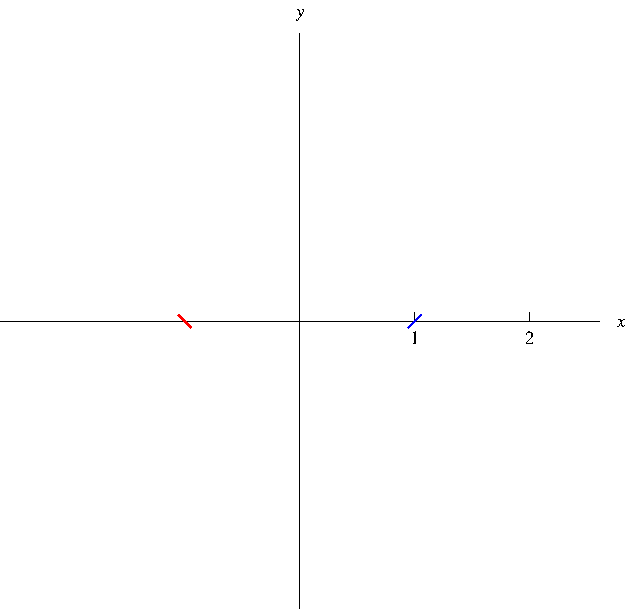
\includegraphics[height=5cm]{diff-eq-direction-fields/pictures/10-02-dirfieldd.pdf}%
%}%
%\only<handout:0| 7>{%
%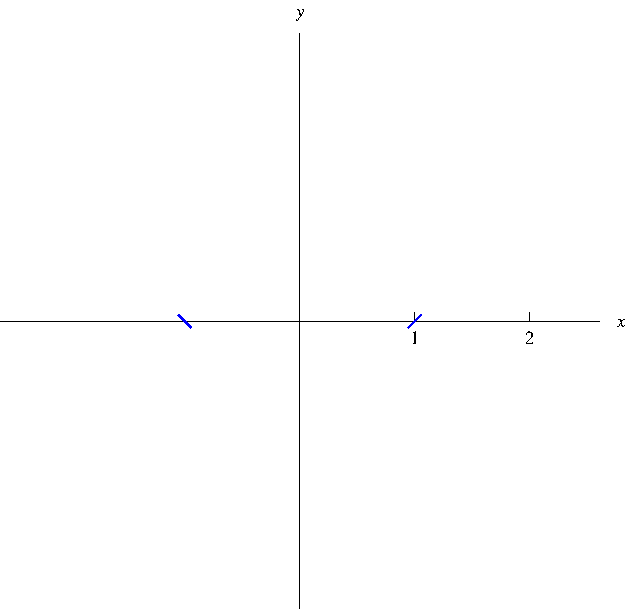
\includegraphics[height=5cm]{diff-eq-direction-fields/pictures/10-02-dirfielde.pdf}%
%}%
%\only<handout:0| 8>{%
%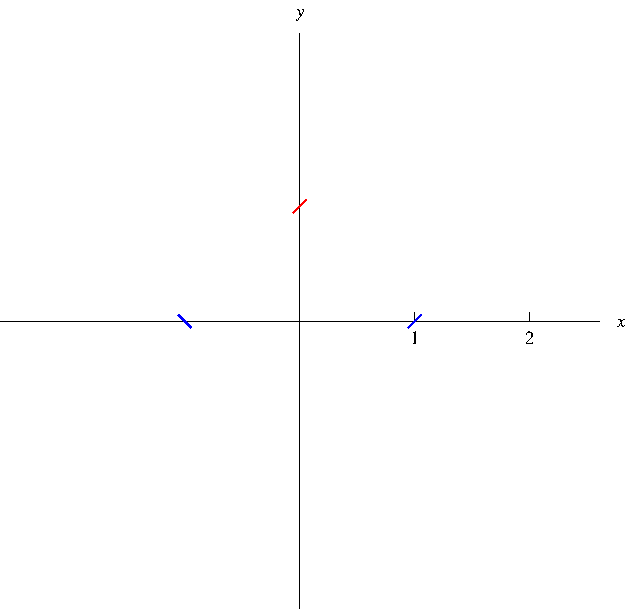
\includegraphics[height=5cm]{diff-eq-direction-fields/pictures/10-02-dirfieldf.pdf}%
%}%
%\only<handout:0| 9>{%
%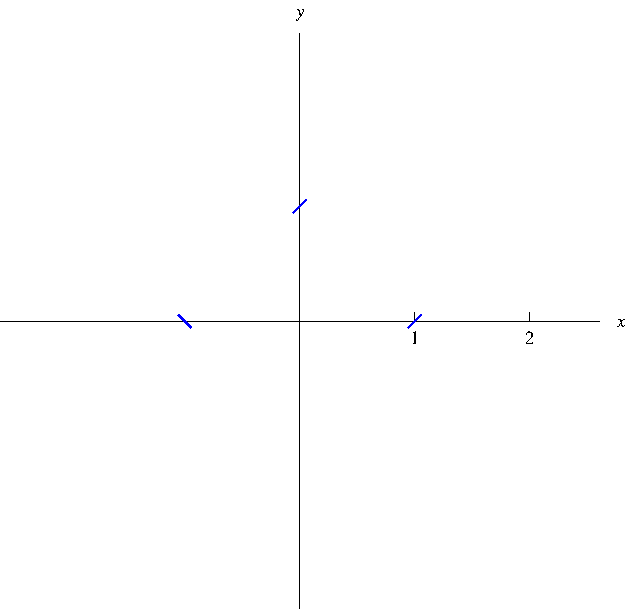
\includegraphics[height=5cm]{diff-eq-direction-fields/pictures/10-02-dirfieldg.pdf}%
%}%
%\only<handout:0| 10>{%
%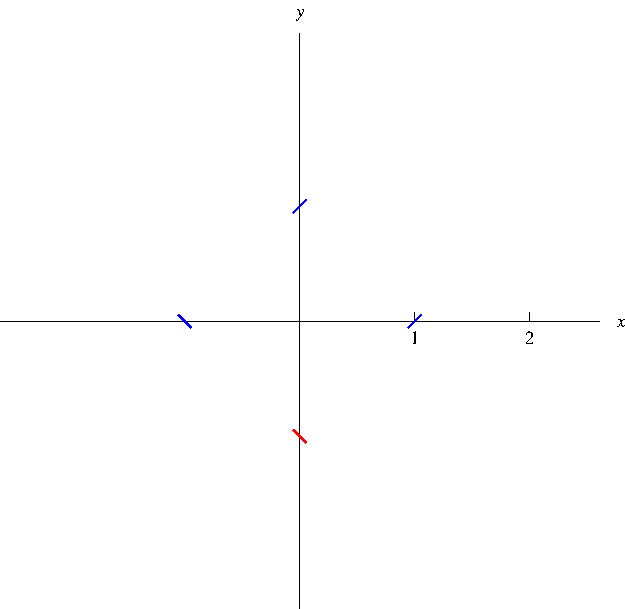
\includegraphics[height=5cm]{diff-eq-direction-fields/pictures/10-02-dirfieldh.pdf}%
%}%
%\only<handout:0| 11>{%
%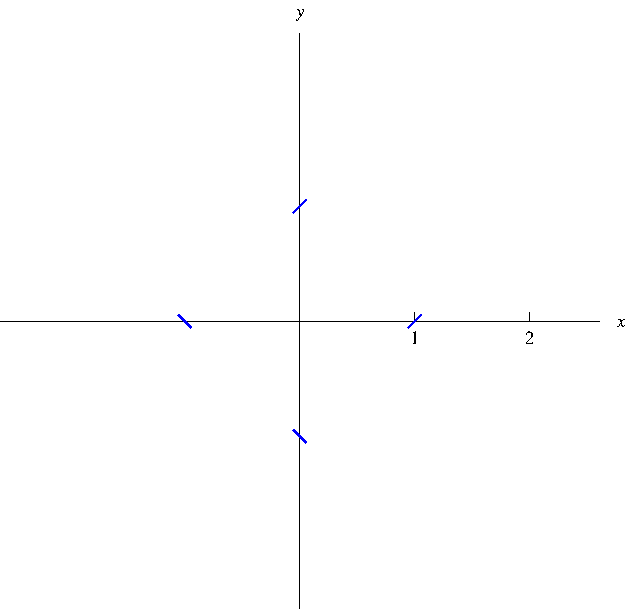
\includegraphics[height=5cm]{diff-eq-direction-fields/pictures/10-02-dirfieldi.pdf}%
%}%
%\only<handout:0| 12>{%
%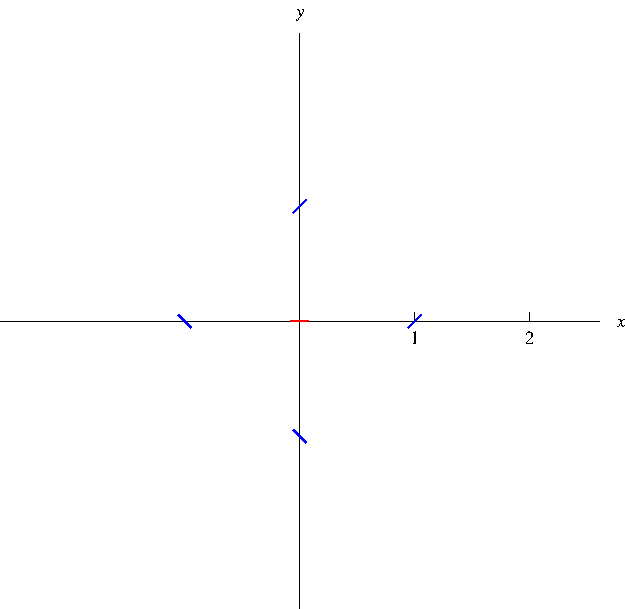
\includegraphics[height=5cm]{diff-eq-direction-fields/pictures/10-02-dirfieldj.pdf}%
%}%
%\only<handout:0| 13>{%
%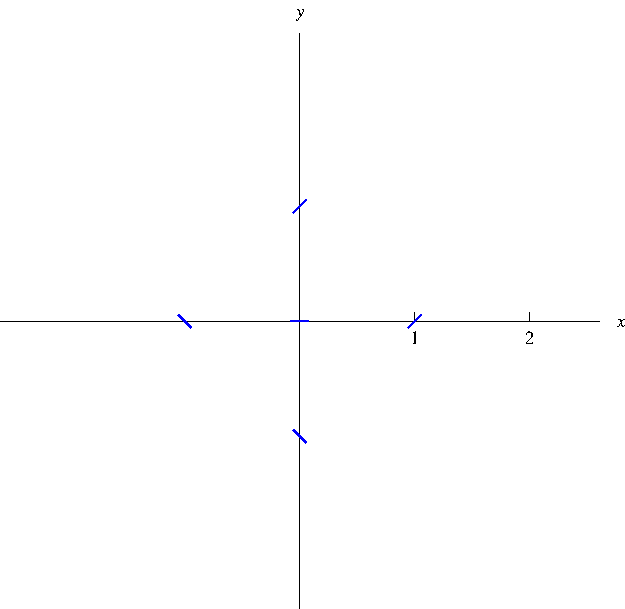
\includegraphics[height=5cm]{diff-eq-direction-fields/pictures/10-02-dirfieldk.pdf}%
%}%
%\only<handout:0| 14>{%
%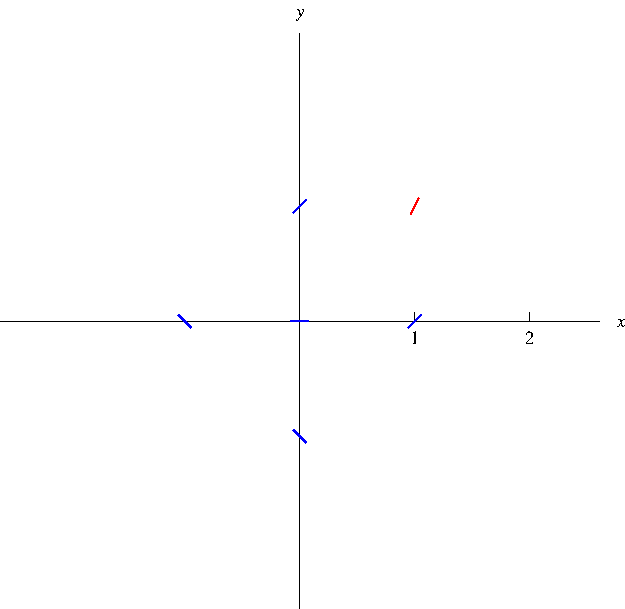
\includegraphics[height=5cm]{diff-eq-direction-fields/pictures/10-02-dirfieldl.pdf}%
%}%
%\only<handout:0| 15>{%
%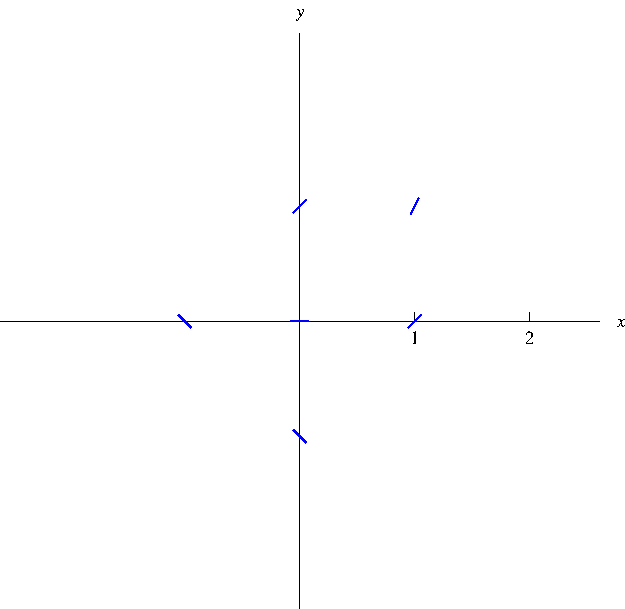
\includegraphics[height=5cm]{diff-eq-direction-fields/pictures/10-02-dirfieldm.pdf}%
%}%
%\only<handout:0| 16>{%
%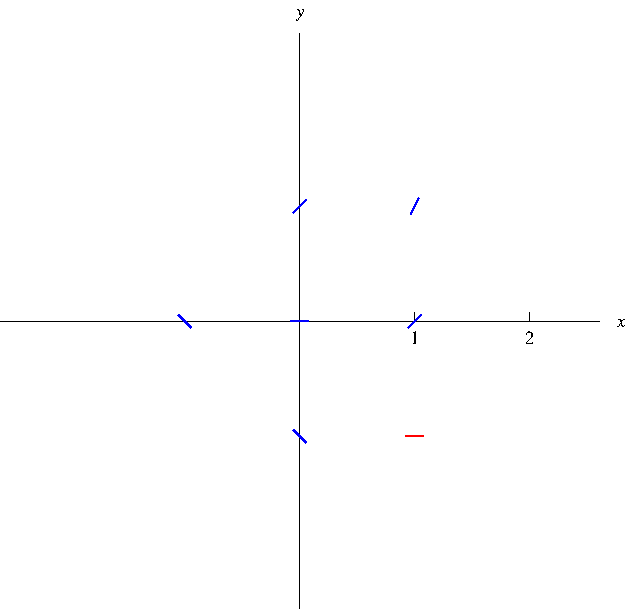
\includegraphics[height=5cm]{diff-eq-direction-fields/pictures/10-02-dirfieldn.pdf}%
%}%
%\only<handout:0| 17>{%
%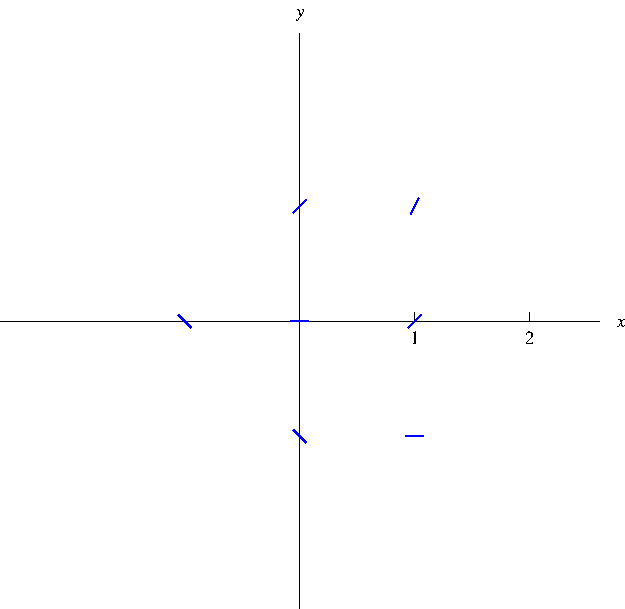
\includegraphics[height=5cm]{diff-eq-direction-fields/pictures/10-02-dirfieldo.pdf}%
%}%
%\only<handout:0| 18>{%
%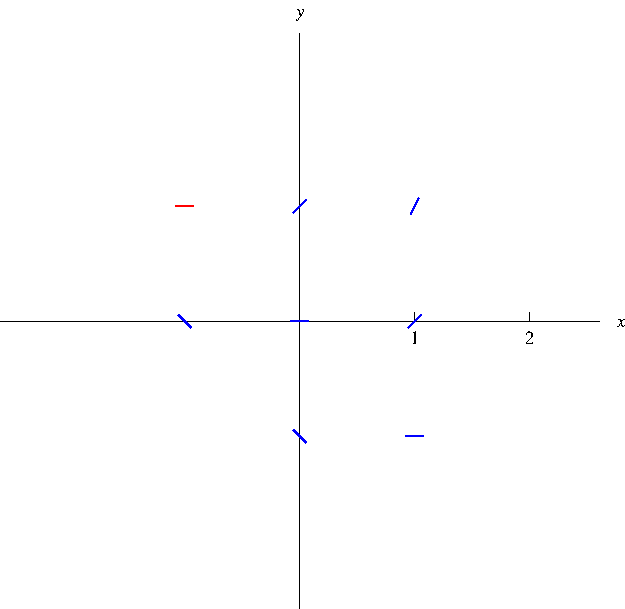
\includegraphics[height=5cm]{diff-eq-direction-fields/pictures/10-02-dirfieldp.pdf}%
%}%
%\only<handout:0| 19>{%
%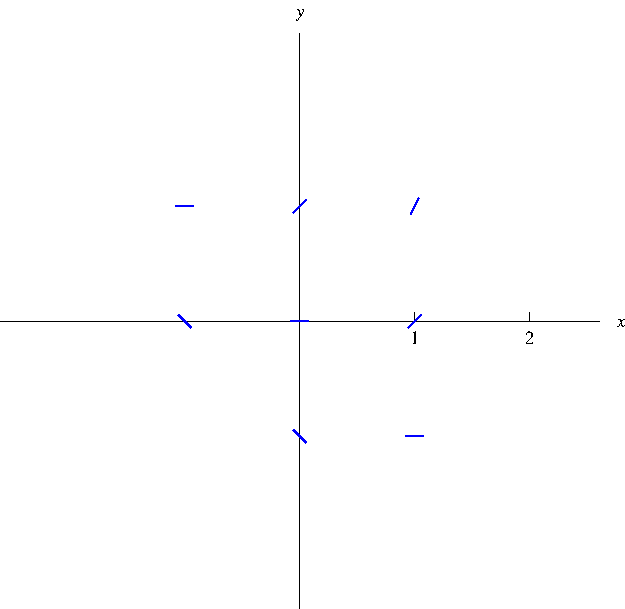
\includegraphics[height=5cm]{diff-eq-direction-fields/pictures/10-02-dirfieldq.pdf}%
%}%
%\only<handout:0| 20>{%
%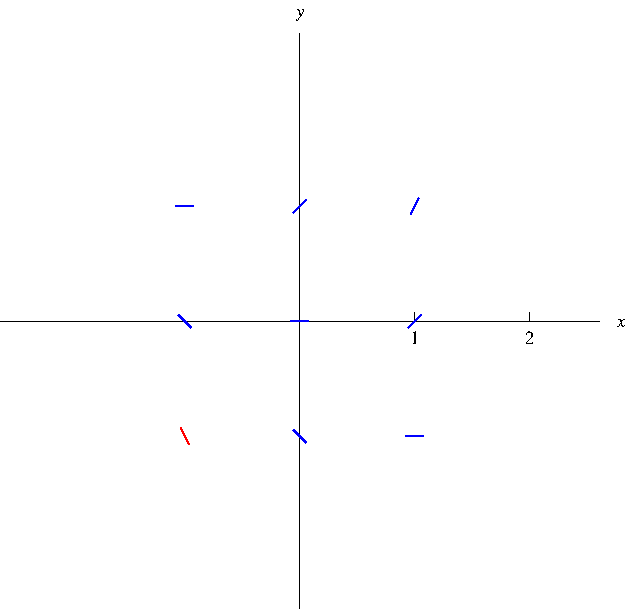
\includegraphics[height=5cm]{diff-eq-direction-fields/pictures/10-02-dirfieldr.pdf}%
%}%
%\only<handout:0| 21-22>{%
%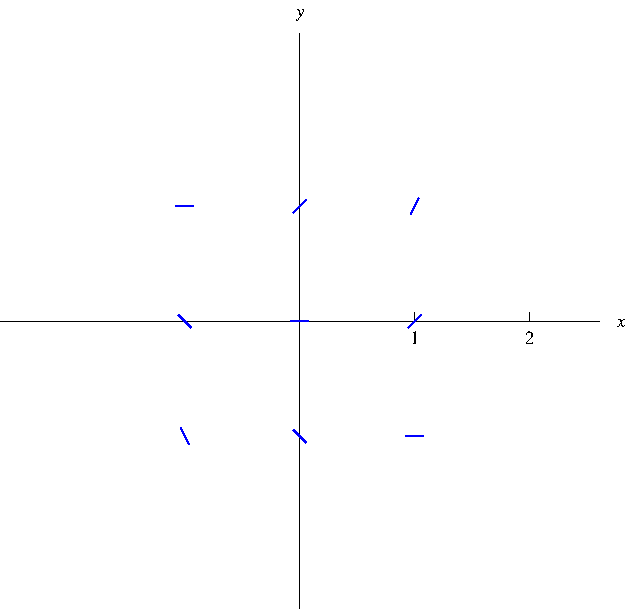
\includegraphics[height=5cm]{diff-eq-direction-fields/pictures/10-02-dirfields.pdf}%
%}%
%\only<handout:0| 23>{%
%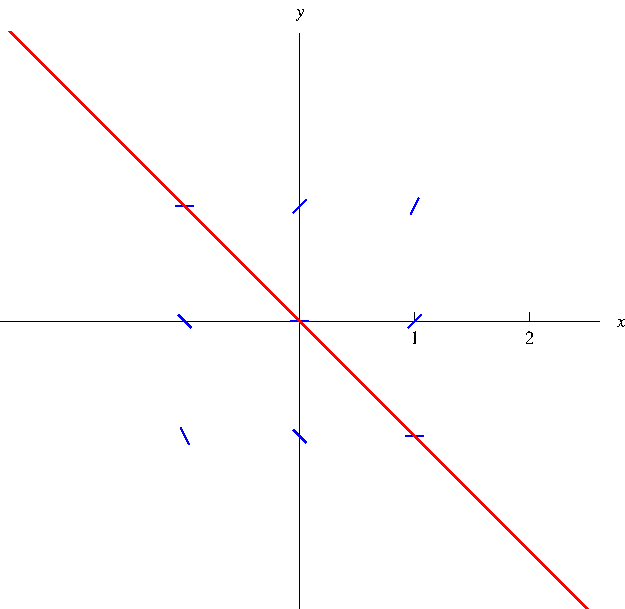
\includegraphics[height=5cm]{diff-eq-direction-fields/pictures/10-02-dirfieldt.pdf}%
%}%
%\only<handout:0| 24>{%
%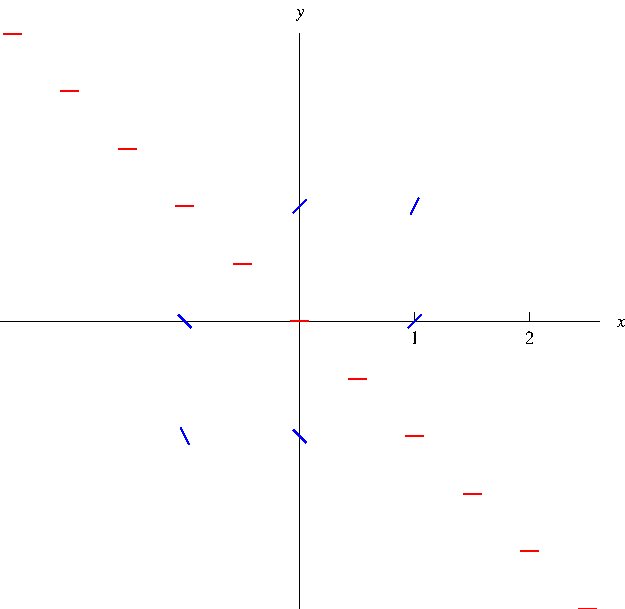
\includegraphics[height=5cm]{diff-eq-direction-fields/pictures/10-02-dirfieldu.pdf}%
%}%
%\only<handout:0| 25>{%
%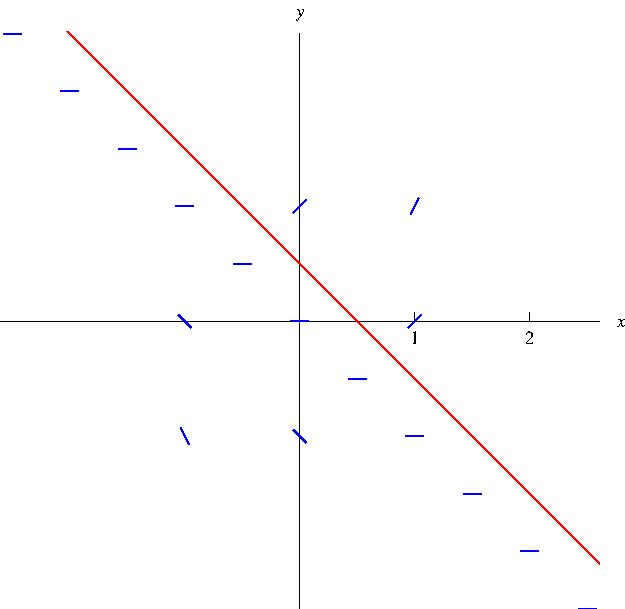
\includegraphics[height=5cm]{diff-eq-direction-fields/pictures/10-02-dirfieldv.pdf}%
%}%
%\only<handout:0| 26>{%
%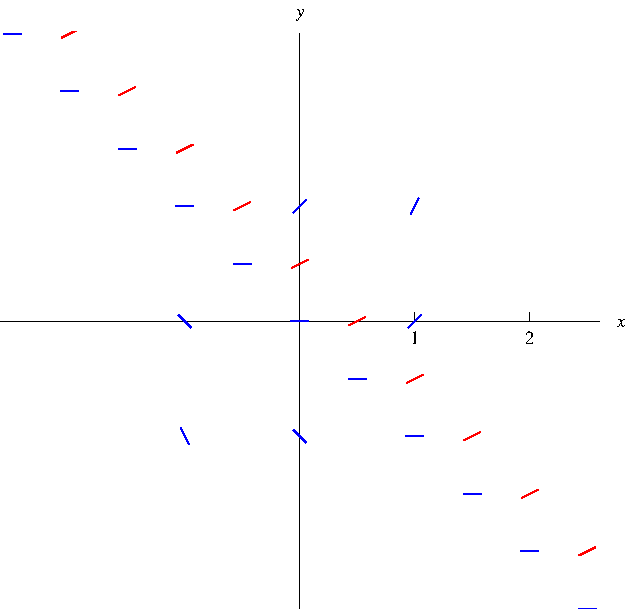
\includegraphics[height=5cm]{diff-eq-direction-fields/pictures/10-02-dirfieldw.pdf}%
%}%
%\only<handout:0| 27>{%
%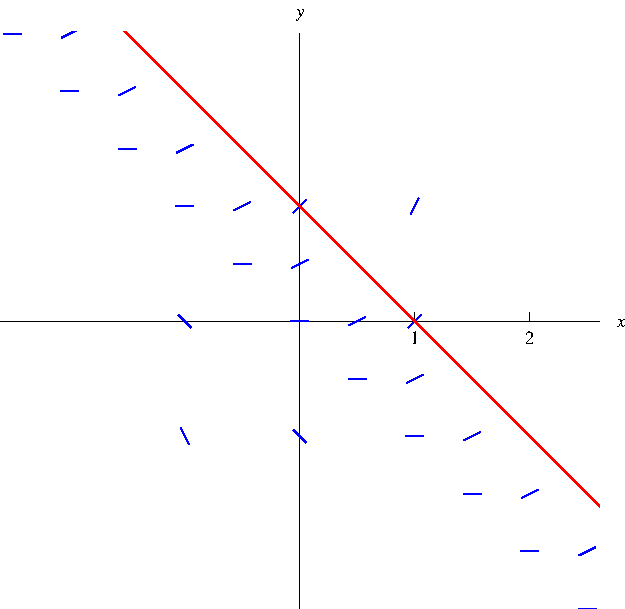
\includegraphics[height=5cm]{diff-eq-direction-fields/pictures/10-02-dirfieldx.pdf}%
%}%
%\only<handout:0| 28>{%
%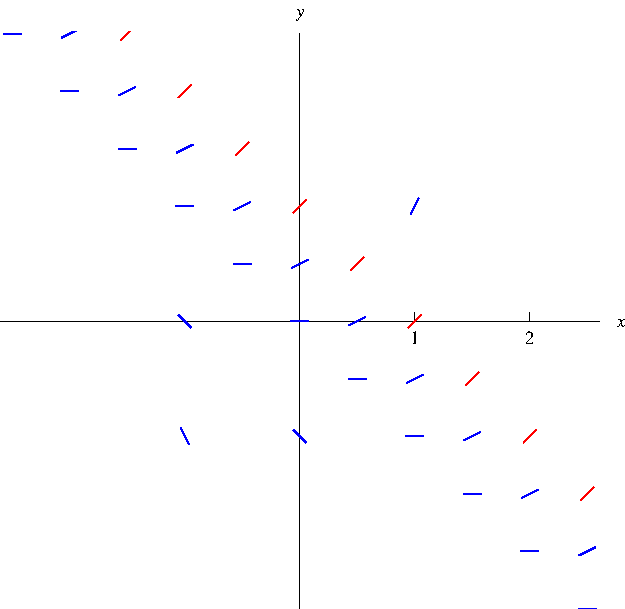
\includegraphics[height=5cm]{diff-eq-direction-fields/pictures/10-02-dirfieldy.pdf}%
%}%
%\only<handout:0| 29>{%
%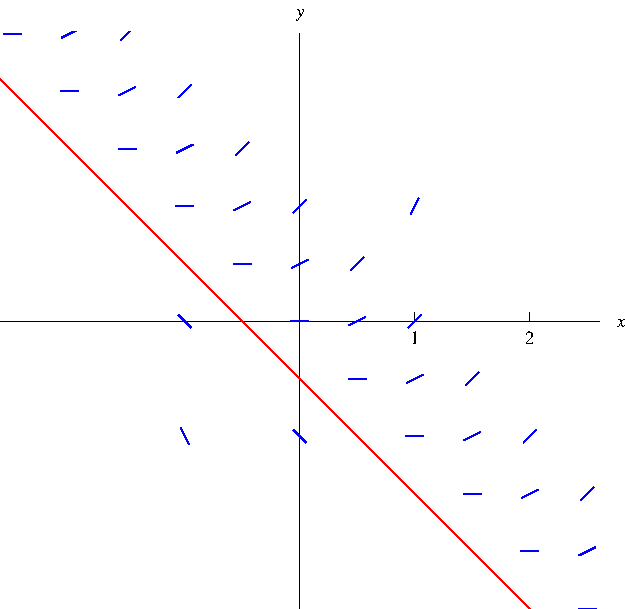
\includegraphics[height=5cm]{diff-eq-direction-fields/pictures/10-02-dirfieldz.pdf}%
%}%
%\only<handout:0| 30>{%
%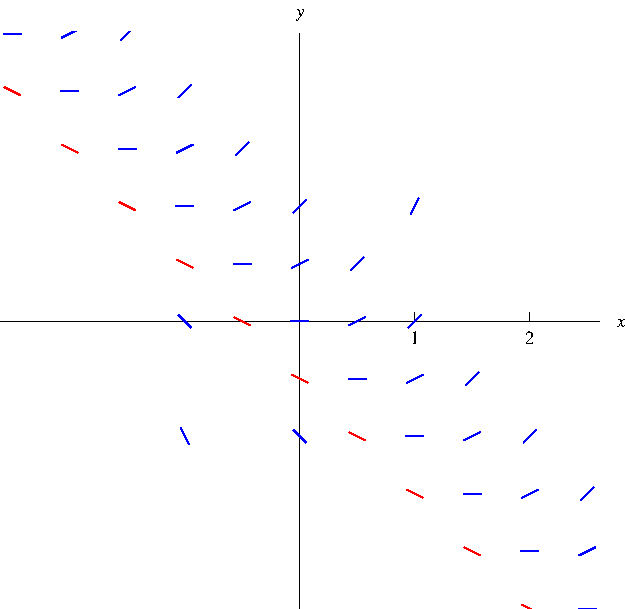
\includegraphics[height=5cm]{diff-eq-direction-fields/pictures/10-02-dirfieldaa.pdf}%
%}%
%\only<handout:0| 31>{%
%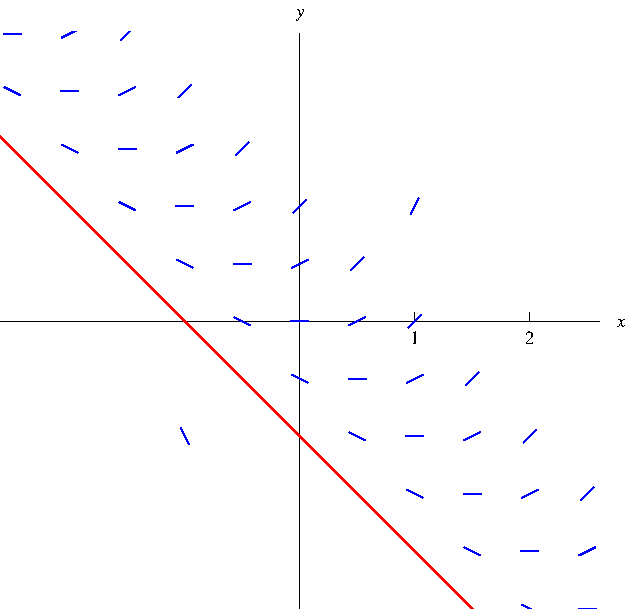
\includegraphics[height=5cm]{diff-eq-direction-fields/pictures/10-02-dirfieldab.pdf}%
%}%
%\only<handout:0| 32>{%
%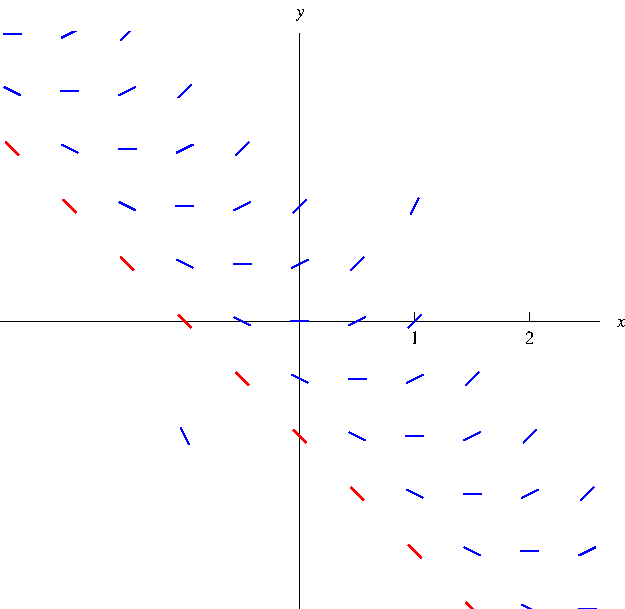
\includegraphics[height=5cm]{diff-eq-direction-fields/pictures/10-02-dirfieldac.pdf}%
%}%
%\only<handout:0| 33>{%
%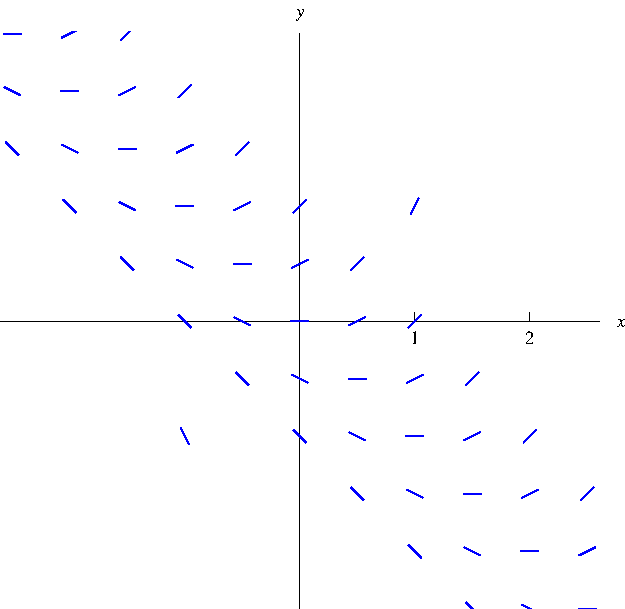
\includegraphics[height=5cm]{diff-eq-direction-fields/pictures/10-02-dirfieldad.pdf}%
%}%
%\only<handout:0| 34>{%
%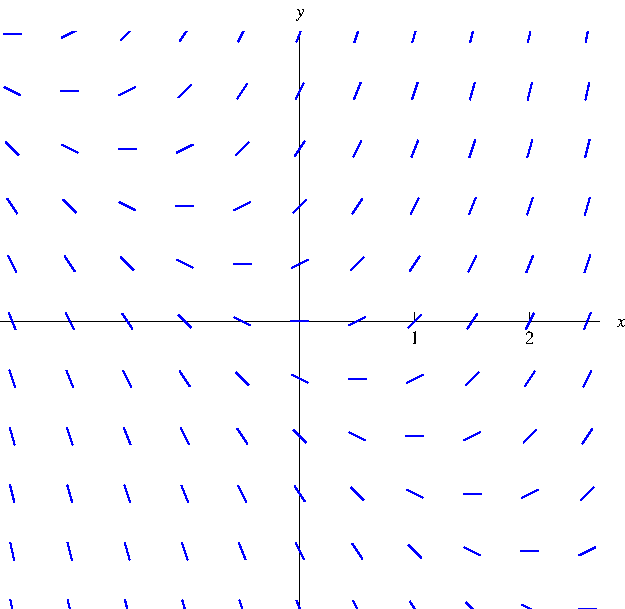
\includegraphics[height=5cm]{diff-eq-direction-fields/pictures/10-02-dirfieldae.pdf}%
%}%
%\only<35>{%
%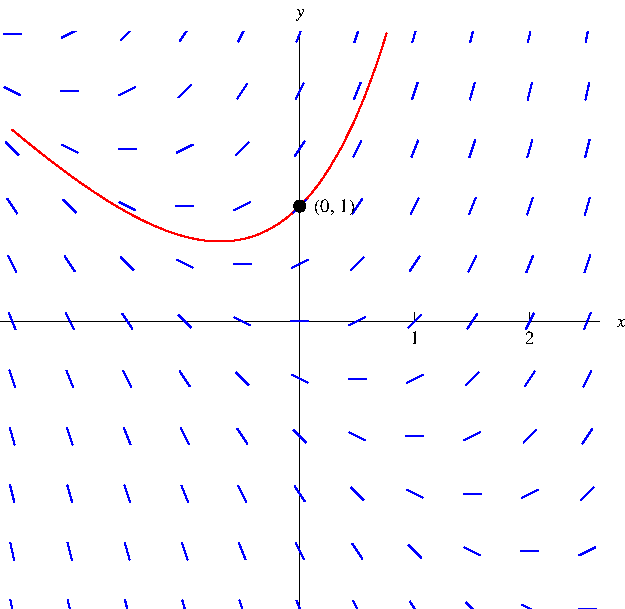
\includegraphics[height=5cm]{diff-eq-direction-fields/pictures/10-02-dirfieldaf.pdf}%
%}%

\column{.3\textwidth}
\uncover<22->{%
\[%
\begin{array}{|l|r|}
\hline
\textrm{Line} & y' \\
\hline
\alert<handout:0| 23-24>{y = -x}&%
\alert<handout:0| 23-24>{\uncover<24->{0}}\\%
\alert<handout:0| 25-26>{y = -x+\frac{1}{2}}&%
\alert<handout:0| 25-26>{\uncover<26->{\frac{1}{2}}}\\%
\alert<handout:0| 27-28>{y = -x+1}&%
\alert<handout:0| 27-28>{\uncover<28->{1}}\\%
\alert<handout:0| 29-30>{y = -x-\frac{1}{2}}&%
\alert<handout:0| 29-30>{\uncover<30->{-\frac{1}{2}}}\\%
\alert<handout:0| 31-32>{y = -x-1}&%
\alert<handout:0| 31-32>{\uncover<32,33,34,35->{-1}}\\%
\hline
\end{array}
\]%
}%
\end{columns}
\end{frame}
% end module direction-fields-procedure
